\documentclass[10pt,journal,compsoc]{IEEEtran}


\usepackage{booktabs} % For formal tables
\usepackage{xspace}
\usepackage{mathtools}
\usepackage{amsthm}
\usepackage{algorithm}
\usepackage{todonotes}
\usepackage{color}
\usepackage{enumitem}
\usepackage{balance}
\usepackage{flushend}
\usepackage[noend]{algpseudocode}
\usepackage{multirow}

% These commands are optional
%\acmBooktitle{Transactions of the ACM Woodstock conference}
%\editor{Jennifer B. Sartor}
%\editor{Theo D'Hondt}
%\editor{Wolfgang De Meuter}

\newcommand{\formal}[1]{\textbf{\textsc{#1}}\xspace}
\DeclarePairedDelimiter{\ceil}{\lceil}{\rceil}
\DeclarePairedDelimiter{\floor}{\lfloor}{\rfloor}

\newtheorem{theorem}{Theorem}
\newtheorem{corollary}{Corollary}
\newtheorem{lemma}{Lemma}
\newtheorem{example}{Example}
\newtheorem{definition}{Definition}

\newcommand{\cudpp}{{\tt CUDPP}\xspace}
\newcommand{\megakv}{{\tt MegaKV}\xspace}
\newcommand{\linear}{{\tt Linear}\xspace}
\newcommand{\google}{{\tt GoogleHash}\xspace}
\newcommand{\voter}{{\tt DynamicVoter}\xspace}

\newcommand{\dstwitter}{{\tt TW}\xspace}
\newcommand{\dsreddit}{{\tt RE}\xspace}
\newcommand{\dstpch}{{\tt LINE}\xspace}
\newcommand{\dsali}{{\tt COM}\xspace}
\newcommand{\dsrandom}{{\tt RAND}\xspace}

\newcommand{\xxx}{\textbf{\color{red}{XXX}}\xspace}


\begin{document}
\title{Dynamic Hash Tables on GPUs}


\author{Yuchen~Li, Jing Zhang, Yue Liu, Zheng Lyu, Zhongdong Huang, Jianling Sun
	\IEEEcompsocitemizethanks{
		\IEEEcompsocthanksitem Y. Li is with the School of Information Systems,
		Singapore Management University.
		E-mail: yuchenli@smu.edu.sg
		\IEEEcompsocthanksitem J. Zhang, Y. Liu, Z. Huang and J. Sun are with the College of Computer Science and Technology, Zhejiang University.
		E-mail: \{zhangjing000, liuyue1013, hzd, sunjl\}@zju.edu.cn
		\IEEEcompsocthanksitem Z. Lyu is with the Alibaba Group.
	}%
}

%\numberofauthors{1}
%\author{
%	\alignauthor
%	Yuchen Li$^\dagger$, Jing Zhang, Yue Liu, Zheng Lyu$^*$, Zhongdong Huang, Jianling Sun\\
%	\affaddr{$^\dagger$Singapore Management University},
%	\affaddr{$^*$Alibaba Group},
%	\affaddr{Zhejiang University}
%	\email{$^\dagger$yuchenli@smu.edu.sg, $^*$lvzheng.lz@alibaba-inc.com, \\
%		\{zhangjing000, liuyue1013, hzd, sunjl\}@zju.edu.cn}
%}


\IEEEtitleabstractindextext{%
\begin{abstract}
The hash table is a fundamental structure that
has been implemented on graphics processing units (GPUs) to accelerate a wide range of analytics workloads. Most existing works have focused on static scenarios and occupying large GPU memory to maximize the insertion efficiency. In many cases, data stored in hash tables get updated dynamically and existing approaches use unnecessarily large memory resources.
One na\"ive solution is to rebuild a hash table (known as rehashing) whenever it is either filled or mostly empty. However, this approach renders significant overheads for rehashing.
In this paper, we propose a novel dynamic cuckoo hash table technique on GPUs, known as \emph{DyCuckoo}. 
We devise a resizing strategy for dynamic scenarios without rehashing the entire table that ensures a guaranteed filled factor.
The strategy trades search performance with resizing efficiency, and this tradeoff can be configured by users.
To further improve efficiency, we propose a two-layer cuckoo hashing scheme that ensures a maximum of \emph{two} lookups for find and delete operations, while retaining similar performance for insertions as a general cuckoo hash. 
Extensive experiments have validated the proposed design's effectiveness over several state-of-the-art hash table implementations on GPUs. 
\emph{DyCuckoo} achieves superior performance while saving up to four times the memory over the state-of-the-art approaches against dynamic workloads.
\end{abstract}
}

\maketitle
\IEEEdisplaynontitleabstractindextext
\IEEEpeerreviewmaketitle

\section{introduction}
Exceptional advances in general-purpose graphics processing units (GPGPUs) 
in recent years have completely revolutionized computing paradigms across multiple fields such as cryptocurrency mining \cite{o2014bitcoin,taylor2013bitcoin}, machine learning \cite{coates2013deep,abadi2016tensorflow}, and database technologies \cite{bakkum2010accelerating,kaldewey2012gpu}.
GPUs bring phenomenal computational power that had previously only been available from supercomputers in the past. 
%The state-of-the-art commercial GPU equipment (GV100) is capable to operate at the speed of 14.8 TFLOPS for single precision arithmetic and 870 GB/s peak memory bandwidth \footnote{Quadro GV100 launched by NVIDIA in March 2018}. 
Hence, there is a prevailing interest in developing efficient parallel algorithms for GPUs to enable real-time analytics.
%Meanwhile, as the computing resources of GPUs continue to explode, it makes rooms for more applications to run on a single GPU equipment concurrently. For example, GV100 is built with 5120 CUDA cores and 32GB device memory. Nevertheless, most GPU programs try to occupy as much resources as possible to maximize their performance individually. 
%The egoism renders inefficiency when the GPUs run multiple programs simultaneously. Imagining a number of concurrent programs requesting a total memory size larger than the device memory. Interleaving the program executions leads to redundant data transfers between CPUs and GPUs through PCIe, which is expensive in nature. 

In this paper, we investigate a fundamental data structure, known as the \emph{hash table}, which has been implemented on GPUs to accelerate applications, ranging from relational hash joins \cite{he2008relational,he2009relational,heimel2013hardware}, data mining \cite{pan2011fast,zhou2010parallel,zhong2014medusa},  key value stores \cite{zhang2015mega,hetherington2015memcachedgpu,breslow2016horton}, and many others \cite{bowers2010parallel,pan2010efficient,garcia2011coherent,niessner2013real,wu2015gpu}. Existing works \cite{alcantara2009real,zhang2015mega,hong2010mapcg,hetherington2015memcachedgpu,breslow2016horton} have focused on static scenarios in which the size of the data is known in advance and  a sufficiently large hash table is allocated to insert all data entries. 
\revise{
However, data size varies in different application scenarios such as sensor data processing, Internet traffic analysis and analysis of transaction logic such as in web server logs and telephone calls. When data size varies, the static allocation strategy leads to poor memory utilization~\cite{ashkiani2018dynamic}. 
}
The static strategy is thus inefficient when an application requires multiple data structures to coexist on GPUs. One must resort to expensive PCIe data transfer between CPUs and GPUs, as the hash table takes up an unnecessarily large memory space. 
Addressing this shortcoming calls for a dynamic GPU hash table that adjusts to the size of active entries in the table. 
Such a hash table should support efficient memory management by sustaining a guaranteed \emph{filled factor} of the table when the data size changes. 
In addition to efficient memory usage, the dynamic approach should retain the performance of common hash table operations such as find, delete, and insert.
\revise{
Although dynamically-sized hash tables have been studied across academia \cite{liu2014dynamic,zuo2018write} and industry \cite{larson2003scaleable,douceur2000hash} for CPUs, 
GPU-based dynamic hash tables have largely been overlooked.}
%Maintaining high hilled factor indicates that the table needs to be frequently adjusted to the active data size and it incurs costly rehashing to move the entries in the hash table.
%There are two major challenges for maintaining a high filled factor for hash tables on GPUs:
%\begin{itemize}
%	\item It leads to a smaller hash table size with less distinct keys, hence triggers additional conflicts as multiple threads trying to insert/delete the data, which is particularly expensive under the GPU architecture;
%	\item It also means that the table needs to be frequently adjusted to the active data size and it incurs costly rehashing to move the entries to a new table when the old table cannot accommodate the adjusted data. 
%\end{itemize}

In this paper, we propose a dynamic cuckoo hash table on GPUs, known as \voter. Cuckoo hashing \cite{pagh2004cuckoo} uses several hash functions to give each key multiple locations instead of one. When a location is occupied, the existing key is relocated to make room for the new one. Existing works \cite{alcantara2009real,alcantara2011building,zhang2015mega,breslow2016horton} have demonstrated great success in speeding up applications using parallel cuckoo hashes on GPUs. 
%However, most of these works require the size of a Key-Value (KV) pair to fit a single atomic transaction on GPUs (64 bits wide) to handle conflicts when multiple threads trying to update keys hashed to the same value.
%They also build on inefficient locking mechanisms to handle conflicts, which severely downgrade the performance when high contention occurs. 
However, a complete relocation of the entire hash table is required when the data cannot be  inserted.
%It thus calls for a general hash table design to support larger KV size as well as efficient relocation strategy against dynamic updates.
In this work, we propose two novel designs for implementing dynamic cuckoo hash tables on GPUs.

First, we employ the cuckoo hashing scheme with $d$ subtables specified by $d$ hash functions, and introduce a resizing policy to maintain the filled factor within a bounded range while minimizing entries in all subtables being relocated at the same time. 
If the filled factor falls out of the specified range, insertions and deletions would cause the hash tables to grow and shrink.
Our proposed policy only locks one subtable for resizing and ensures that no subtable can be more than twice as large as any other to efficiently handle subsequent resizing. Meanwhile, the hash table entries are distributed to give each subtable a nearly equivalent filled factor.
In this manner, we drastically reduce the cost of resizing hash tables and provide better system availability than the static strategy, which must relocate all data for resizing.
Our theoretical analysis demonstrates the scheduling policy's optimality in terms of processing updates. 

Second, we propose a two-layer cuckoo hashing scheme to ensure efficient hash table operations. 
The proposed resizing strategy requires $d$ hash tables, which indicates $d$ lookup positions for find and delete operations, and a larger $d$ indicates less workload for resizing but more lookups for find and delete operations. To mitigate this tradeoff, we devise a two-layer approach that first hashes any key to a pair of hash tables where the key can be further hashed and stored in one of the two hash tables.  
This design ensures that there are a maximum of two lookups for any find and deletion operations.
%which is pivotal for GPU architecture as random lookups are particularly expensive due to small cache sizes and simplified control units.
Furthermore, the two-layer approach retains the general cuckoo hash tables' performance guarantee.
Empirically, the proposed hash table design can operate efficiently at filled factors exceeding 90\%.

%Second, we propose a voter-based coordination scheme among massive GPU threads to support efficient locking without assuming the size of the key-value pairs.
%For each hash value, we allocate a bucket of $b$ locations to store key-value pairs. 
%Each thread is assigned to an insertion operation on one key. Instead of immediately acquiring a lock on the corresponding bucket to be updated, a thread will first propose a vote among its warp group and all threads in that same warp collaborate to join the winner thread for its update task. There are three distinguishing advantages for the voter-based coordination: (a) once a conflict is detected on one bucket, instead of spinning, the warp instantly revotes and switches to another bucket; (b) a near-optimal load balancing is achieved as a thread will assist other warp-aligned threads, even when the thread finishes its assigned tasks; (c) locking the bucket exclusively allows to update KV pairs without assuming their length below 64 bits.

Thus, we summarize our contributions as follows:
\begin{itemize}
%	\item We propose a general dynamic hash table without assuming the size of the key-value pair and devise a novel voter-based coordination scheme to support the locking mechanism under massive GPU threads. 
	\item We propose an efficient strategy for resizing hash tables and demonstrate the near-optimality of the resizing strategy through theoretical analysis.
	\item We devise a two-layer cuckoo hash scheme that ensures a maximum of two lookups for find and deletion operations, while still retaining similar performance for insertions as general cuckoo hash tables. 
	\item We conduct extensive experiments on both synthetic and real datasets and compare the proposed approach against several state-of-the-art GPU hash table baselines. For dynamic workloads, the proposed approach demonstrates superior performance and reduces memory usage by up to a factor of four over the compared baselines.
\end{itemize}

The remainder of this paper is organized as follows. Section~\ref{sec:pre} introduces the preliminary information and provides a background on GPUs. 
Section~\ref{sec:rel} documents related work.
Section~\ref{sec:dyn} introduces the hash table design and the resizing strategy against dynamic updates.
Section~\ref{sec:vot} presents the two-layer cuckoo hash scheme along with parallel operations on GPUs. The experimental results are reported in Section~\ref{sec:exp}. Finally, we conclude the paper in Section~\ref{sec:con}.
\section{preliminaries}\label{sec:pre}
In this section, we first introduce some preliminaries on general hash tables and then present the background on the GPU architecture. 

\begin{table}
	\centering
	\caption{Frequently Used Notations}
	\vspace{-1.5em}
	\label{tbl:stat:datasets}
	\begin{tabular}{|c|l|}
		\hline
		$(k,v)$ & a key value pair \\ \hline
		$d$		& the number of hash functions \\ \hline
		$h^i$	& the $i$th hash table \\ \hline
		$|h^i|,n_i,m_i$	& range, table size and data size of $h^i$ \\ \hline
		$wid,l$	& a warp ID and the $l$th lane of the warp \\ \hline
		$\theta$& filled factor of the entire hash table \\ \hline
		$\theta_i$& filled factor of hash table $i$ \\ \hline
		$loc$	& a bucket in the hash table \\ \hline
	\end{tabular}
\end{table}

\subsection{Hash Table}
A hash table is a fundamental data structure to store KV pairs $(k,v)$ and the value could refer to either the actual data or a reference to the data.
The hash table offers the following functionalities: \formal{insert}$(k,v)$ - stores $(k,v)$ in the hash table; \formal{find}$(k)$ - given $k$ returns the associated values if they exist, and NULL otherwise; and \formal{delete}$(k)$ - removes existing KVs that match $k$ if they present in the table.

Given a hash function with range $0 \ldots h-1$, collisions must happen when we insert $m>h$ keys into the table. There are many schemes to resolve collisions: linear probing, quadratic probing, chaining and etc. Contrary to these schemes, cuckoo hashing \cite{pagh2004cuckoo} guarantees a worst case constant complexity for \formal{find} and \formal{delete},  and an amortized constant complexity for \formal{insert}. A cuckoo hash uses multiple (i.e., $d$) hash tables with independent hash functions $h^1,h^2,\ldots,h^d$ and stores a KV in \emph{one} of the hash tables. When inserting a $(k,v)$, we store the pair to $loc=h^1(k)$ and terminate if there is no element at this location. Otherwise, if there exists $k'$ such that $h^1(k')=loc$, $k'$ is evicted and will be reinserted into another hash table, e.g., $loc'=h^2(k')$.
We repeat this process until an empty location is encountered.

For a hash table with the hash function $h^i$, $|h^i|$ is defined to be the number of unique hash values for $h^i$ and $n_i$ to be the total memory size allocated for the hash table.
A location or a hash value for $h^i$ is represented as $loc = h^i_j$ where $j \in [0,|h^i|-1]$.
If the occupied space of the hash table is $m_i$, the filled factor of $h^i$ is denoted as $\theta_i = m_i / n_i$. The overall filled factor of the cuckoo hash table is denoted as $\theta = (\sum_i m_i) / (\sum_i n_i)$.

\subsection{GPU Architecture}

\begin{figure}[t]
	\centering
	\includegraphics[width=0.5\textwidth]{fig/GPU-arch.pdf}
	\caption{Layout of an NVIDIA GPU architecture}
	\label{fig:arch}
\end{figure}

We focus on introducing the background of NVIDIA GPU architecture in this paper due to its popularity and wide adoption of the CUDA programming language. 
It is noted that our proposed approaches are not unique to NVIDIA GPUs and can be implemented on other GPU architectures as well. Figure~\ref{fig:arch} presents a high-level layout of a NVIDIA GPU. An application written in CUDA executes on GPUs through invoking the \emph{kernel} function. The kernel is organized as a number of \emph{thread blocks}, and one block executes all its threads on a \emph{streaming multiprocessor}, which contains a number of CUDA cores as depicted in the figure. Within a block, threads are divided into \emph{warps} of 32 threads each. 
A CUDA core executes the same instruction of a warp in a lockstep.
Each warp runs independently but can collaborate through different memory types discussed as the following.  

\vspace{1mm}\noindent\textbf{Memory Hierarchy.} Compared CPUs, GPUs are built with large register files to enable massive parallelism. 
For example, NVIDIA GTX 1080 GPUs feature 256KB of register files for each SM. Furthermore, the shared memory, which has similar performance with the L1 cache, can be programmed within a block to facilitate efficient local memory access inside a SM.
The L2 cache is shared among all SMs to speedup memory access to the device memory. The device memory has the largest capacity and the lowest bandwidth in the GPU memory hierarchy.

%GPUs offer an significant better data accessing throughputs than CPUs for two major reasons. 
%First,the device memory has high memory bandwidth, often an order of magnitude faster than RAM.
%Second, GPUs effectively hide memory access latency by warp switching. When a warp is blocked by memory accesses, other warps whose next instruction has its operands ready are eligible to be scheduled for execution. With sufficient threads launched, memory stalls can be minimized or even eliminated \cite{zhang2015mega}.
%Thus, the fast data accessing performance makes GPUs an ideal accelerator for data intensive applications such as hash tables. 

%Data is transferred between CPUs and GPUs (or between two GPU devices) via the PCIe link (Gen 3), which has been the bottleneck of many data-intensive applications \cite{zhang2015mega,kaldewey2012gpu,zhang2013omnidb}. In recent years, there have been many innovations proposed to reduce the overhead of the data transfer, from overlapping PCIe transfer with kernel execution to using hardware acceleration such as PCIe Gen 4 and NVlink \cite{thompto2016power9}. Nonetheless, we omit the discussion on how to minimize this data transfer cost since it is orthogonal to designing an efficient hash table on \emph{one} GPU device.

\vspace{1mm}\noindent\textbf{Optimizing GPU Programs.}
When programming a GPU device, there are several important guidelines to harness GPUs' massive parallelism.
\begin{itemize}
	\item \emph{Minimize Warp Divergence.} Threads in a warp will be serialized if they execute different instructions. To enable maximum parallelism, one needs to minimize branching statements executed within a warp.  
	\item \emph{Coalesced Memory Access.} Warps have a wide cache line size (128 bytes for NVIDIA GPU). The threads are better off to read consecutive memory locations for fully utilizing the device memory bandwidth, otherwise to trigger multiple random accesses for a single read instruction by a warp. 
	\item \emph{Control Resource Usage.} Registers and shared memory are valuable resources to enable fast local memory accesses. Nevertheless, each SM has limited resources (GTX 1080 has 98 KB shared memory and 256KB register files per SM). Overdosing register files or shared memory leads to reduced parallelism on a SM.  
	\item \emph{Atomic Operations.} When facing thread conflicts, an improper locking implementation leads to serious performance degradation. One can leverage the native support of atomic operations \cite{sanders2010cuda} on GPUs to carefully resolve the conflicts and minimize thread spinning.
\end{itemize}
\section{related works}\label{sec:rel}
Alcantara \textit{et al.} \cite{alcantara2009real} presented a seminar work on GPU-based cuckoo hashing to accelerate computer graphics workloads. 
This work has inspired several applications from diverse fields. Wu \textit{et al.} \cite{wu2015gpu} investigated the use of GPU-based cuckoo hashing for on-the-fly model checking. 
A proposal of accelerating the nearest neighbor search is presented in \cite{pan2010efficient}. 
Because of the success of cuckoo hashing on GPUs, the implementation of \cite{alcantara2009real} has been adopted in the CUDPP library\footnote{https://github.com/cudpp/cudpp}.
To improve on \cite{alcantara2009real}, stadium hash was proposed in \cite{khorasani2015stadium} to support out-of-core GPU parallel hashing. However, this technique uses double hashing which must rebuild the entire table for any deletions.  
Zhang \textit{et al.}~\cite{zhang2015mega} proposed another efficient design of GPU-based cuckoo hashing, named MegaKV, 
to boost the performance for KV store. 
Subsequently, Horton table \cite{breslow2016horton} improves the efficiency of \formal{find} over MegaKV by trading with the cost of introducing a KV remapping mechanism.
WarpDrive \cite{junger2018warpdrive} employs cooperative groups and multi-GPUs to further improve efficiency.
Meanwhile, in the database domain, several SIMD hash table implementations have been proposed to facilitate relation join and graph processing \cite{ross2007efficient,zhong2014medusa}. 

It is noted that these works have focused on the static case: the data size for insertion is known in advance. The static design would prepare a large enough memory size to store the hash table. In this manner, hash table operations are fast as collisions rarely happen. However, the static approach wastes memory resources and, to some extent, prohibits coexistence with other data structures for the same application in the device memory. 
%Moreover, existing designs rely on atomicExch
%operation to avoid conflicts when transacting a KV pair on GPUs, which only supports up to 64 bits for KV altogether. This design, albeit being efficient, has severe limitation as the value component exceeds 64 bits in many real-world scenarios.  
This motivates us to develop a general dynamic hash table for GPUs that actively adjusts based on the data size to preserve space efficiency. 
%In this paper, we propose a dynamic cuckoo hash table on GPUs, which maintains high filled factor to minimize memory footprint. In order to support efficient concurrent hash updates, we introduce a novel voter-based coordination scheme which reduces thread conflicts. 
%Experimental results have revealed that the proposed solution could achieve competitive or even better performance than the state-of-the-art static hash tables on GPUs, while utilizing significantly less device memory. 

To the best of our knowledge, there is only one existing work on building dynamic hash tables on GPUs \cite{ashkiani2018dynamic}.
This proposed approach presents a concurrent linked list structure, known as \emph{slab list}, to construct the dynamic hash table with \emph{chaining}. 
However, there are three major issues for slab lists.
First, they can frequently invoke concurrent memory allocation requests, especially when the data keeps inserting. Efficient concurrent memory allocation is difficult to implement in a GPU due to its massive parallelism. Although a dedicated memory management strategy to alleviate this allocation cost is proposed in \cite{ashkiani2018dynamic}, the strategy is not transparent to other data structures. More specifically, the dedicated allocator still has to reserve a large amount of memory in advance to prepare for efficient dynamic allocation, and that occupied memory space cannot be readily accessed by other GPU-resident data structures. 
Second, a slab list does not guarantee a fixed filled ratio against deletions. 
It symbolically marks a deleted entry without physically freeing the memory space. 
Hence, memory spaces are wasted when occupied by deleted entries. 
Third, the chaining approach has a lookup time of $\Omega(log(log(m)))$ for some KVs with high probability. This not only results in degraded performance for \formal{find}, it also triggers more overhead for resolving conflicts when multiple \formal{insert} and \formal{delete} operations occur at the same key.
In contrast, the cuckoo hashing table adopted in this work guarantees $\Theta(1)$ worst case complexity for \formal{find} and \formal{delete}, 
and $O(1)$ amortized \formal{insert} performance. Moreover, we do not introduce extra complication in implementing a customized memory manager, but rather rely on the default memory allocator provided by CUDA, while at the same time, ensuring fixed filled ratio for the hash table.
\section{Dynamic Hash Table}\label{sec:dyn}
In this section, we propose a resizing strategy against dynamic hash table updates on GPUs. We first present the hash table design in Section~\ref{sec:dyn:has}.
Subsequently, the resizing strategy is introduced in Section~\ref{sec:dyn:resize}.
In Section~\ref{sec:dyn:distribute}, we discuss how to distribute KV pairs for better load balancing with theoretical guarantees. 
Lastly, we present how to efficiently rehash and relocate data after the tables have been resized in Section~\ref{sec:dyn:rehash}. 

\subsection{Hash Table Structure}\label{sec:dyn:has}
Following cuckoo hashing \cite{pagh2004cuckoo}, we build $d$ hash tables with $d$ unique hash functions: $h^1,h^2,\ldots,h^d$. 
In this work, we use a set of simple universal hash functions such as $h^i(k) = (a_i\cdot k + b_i \mod p) \mod |h^i|$.
Here $a_i,b_i$ are random integers and $p$ is a large prime.
The proposed approaches in this paper also apply to other hash functions as well. 
There are three major advantages of adopting cuckoo hashing on GPUs. 
First, it avoids chaining by inserting the elements into alternative locations if collisions occur. As discussed in Section~\ref{sec:rel}, 
chaining presents several issues that are not friendly to GPU architecture.  
Second, to look up a KV pair, one searches only $d$ locations as specified by $d$ unique hash functions. 
Thus, the data could be stored contiguously in the same location to enable preferred coalesced memory access. 
Third, cuckoo hashing can maintain a high filled factor, which is ideal for saving memory in dynamic scenarios. 
For $d=3$, cuckoo hashing achieves a filled factor of more than 90\% and still efficiently processes \formal{insert} operations \cite{fotakis2005space}.

\begin{figure}[t]
	\centering
	\includegraphics[width=0.45\textwidth]{fig/Hashtable.pdf}
	\caption{The hash table structure}
	\label{fig:hashtable}
\end{figure}

Figure~\ref{fig:hashtable} depicts the design of a single hash table $h^i$ on GPUs. 
The keys are assumed to be 4-byte integers and a bucket of 32 keys, which are all hashed to the same value $h^i_j$, are stored consecutively in the memory. 
The design of buckets maximizes memory bandwidth utilization in GPUs. 
Consider that the L1 cache line size is 128 bytes. Only a single access is required when one warp is assigned to access a bucket. 
The values associated with the keys in the same bucket are also stored consecutively, but in a separate array.  
In other words, we use two arrays, one to store the keys and one to store the values respectively.
However, the values can take up a much larger memory space than the keys; therefore storing keys and values separately avoids memory access overhead when it is not necessary to access the values, such as when finding a nonexistent KV pair or deleting a KV pair. 

For keys larger than 4 bytes, a simple strategy is to store fewer KV pairs in a bucket. If keys are 8 bytes, a bucket can then accommodate 16 KV pairs. 
Furthermore, we lock the entire bucket exclusively for a warp to perform insertions and deletions using intra warp synchronization primitives. Thus, we do not limit ourselves to supporting KV pairs with only 64 bits. 
In the worst case, a key taking 128 bytes would occupy one bucket, which is unnecessarily large in practice.

\subsection{Structure Resizing}\label{sec:dyn:resize}
To efficiently utilize GPU memory, we resize the hash tables when the filled factor falls out of the desired range $[\alpha,\beta]$.
One possible strategy to address this is to double or half all hash tables and rehash all KV pairs. However, this simple strategy renders poor memory utilization and 
excessive rehashing overhead. First, doubling hash table size results in the filled factor being immediately cut in half, whereas downsizing hash tables to half the original size followed by rehashing is only efficient when the filled factor is significantly low (e.g., $40\%$). Both scenarios are not resource friendly. Second, rehashing all KV pairs is expensive and it harms the performance stability for most streaming applications as the entire table is subject to locking. 

Thus, we propose an alternative strategy, illustrated in Figure~\ref{fig:example-resize}.
Given $d$ hash tables,
we always double the smallest subtable or chop the largest subtable in half for upsizing or downsizing, respectively, when the filled factor falls out of the desired range. 
In other words, no subtable will be more than twice the size of others. This strategy implies that we do not need to lock all hash tables to resize only one, thus achieving better performance stability than the aforementioned simple strategy. 


\vspace{1mm}
\noindent\textbf{Filled factor analysis:}
Assuming there are $d'$ hash tables with size $2n$, $d-d'$ tables with size $n$ and a current filled factor of $\theta$, 
one upsizing process when $\theta > \beta$ lowers the filled factor to $\frac{\theta\cdot(d+d')}{d+d'+1} \geq \frac{\beta \cdot d}{d+1}$.  
Because the filled factor is always lower bounded by $\alpha$, we can deduce that $\alpha < \frac{d}{d+1}$.
Apparently, a higher lower bound can be achieved by adding more hash tables, although it leads to less efficient \formal{find} and \formal{delete} operations. 
We allow the user to configure the number of hash tables to trade off memory and query processing efficiency. 

\begin{figure}[t]
	\centering
	\includegraphics[width=0.32\textwidth]{fig/MultiTable.pdf}
	\caption{The resizing strategy}
	\label{fig:example-resize}
\end{figure}
\subsection{KV distribution}\label{sec:dyn:distribute}
Given a set of KV pairs to insert in parallel, it is critical to distribute those KV pairs among the hash tables in a way that minimizes hash collisions to reduce the corresponding thread conflicts. We have the following theorem to guide us in distributing KV pairs. 

\begin{theorem}\label{them:balance}
	The amortized conflicts for inserting $m$ unique KV pairs to $d$ hash tables are minimized when $\binom{m_1}{2}/n_1 = \ldots = \binom{m_d}{2}/n_d$. 
	$m_i$ and $n_i$ denote the elements inserted to table $i$ and the size of table $i$, respectively.  
\end{theorem}
\begin{proof}
	The amortized insertion complexity of a cuckoo hash is $O(1)$. Thus, like a balls and bins analysis, the expected number of conflicts occurring when inserting $m_i$ elements in table $i$ can be estimated as $\binom{m_i}{2}/n_i$. Minimizing the amortized conflicts among all hash tables can be modeled as the following optimization problem:
	\begin{equation}\label{eq:conflict-min}
	\begin{array}{ll@{}ll}
	\min_{m_1,\ldots,m_d \geq 0} & \sum_{i=1,\ldots,d} \binom{m_i}{2}/n_i \\
	\text{s.t.} & \sum_{i=1,\ldots,d} m_i = m
	\end{array}
	\end{equation}
	To solve the optimization problem, we establish an equivalent objective function:
	\begin{align*}
	\min \sum_{i=1,\ldots,d} \frac{\binom{m_i}{2}}{n_i} \Leftrightarrow \min \log(\frac{1}{d}\sum_{i=1,\ldots,d} \frac{\binom{m_i}{2}}{n_i})
	\end{align*}
	According to the Jensen's inequality, the following inequality holds:
	\begin{align*}
	\log(\frac{1}{d}\sum_{i=1,\ldots,d} \frac{\binom{m_i}{2}}{n_i}) \geq \frac{1}{d}\sum_{i=1,\ldots,d}\log(\frac{\binom{m_i}{2}}{n_i})
	\end{align*}
	where equality holds when $\binom{m_i}{2}/n_i = \binom{m_j}{2}/n_j$ $\forall i,j = 1,\ldots,d$ and we obtain the minimum.
\end{proof}

Based on our resizing strategy, one hash table can only be twice as large as the other tables. 
This implies that the filled factors of two tables are equal if they have the same size, i.e., $\theta_i = \theta_j$ if $n_i = n_j$, 
while $\theta_i \simeq \sqrt{2}\cdot \theta_j$ if $n_i = 2n_j$. 
Thus, larger tables should have a higher filled factor. 
Following Theorem~\ref{them:balance},
we employ a randomized approach: 
a KV pair $(k,v)$ is first assigned to table $i$ with a proportional probability to $n_i/\binom{m_i}{2}$ to ensure the distribution of KVs.

\subsection{Rehashing}\label{sec:dyn:rehash}
Whenever the filled factor falls out of the desired range, rehashing relocates KV pairs after one of the hash tables is resized. An efficient relocation process maximizes GPU device memory bandwidth and minimizes thread conflicts. 
We discuss two scenarios for rehashing: \emph{upsizing} and \emph{downsizing}, both of which are processed in a single kernel. 

\begin{figure}[t]
	\centering
	\includegraphics[width=0.3\textwidth]{fig/Upsize.pdf}
	\caption{Illustration for upsizing and downsizing.}
	\label{fig:upsize}
\end{figure}
\vspace{1mm}\noindent\textbf{Upsizing.} 
Here, we introduce a conflict-free rehashing strategy for the upsizing scenario. 
Figure~\ref{fig:upsize} illustrates the upsizing of a hash table $h^i$. 
As we always double the size for $h^i$, 
a KV pair that originally resides in bucket $loc$ could be rehashed to bucket $loc+|h^i|$ or stay in the original bucket. 
With this observation, we assign a warp for rehashing all KV pairs in the bucket to fully utilize the cache line size. 
Each thread in the warp takes a KV pair in the bucket and, if necessary, relocates that KV pair.
Moreover, rehashing does not trigger any conflicts as KV pairs from two distinct buckets before upsizing cannot be rehashed to the same bucket.  
Thus, locking of the bucket is not required, meaning we can make use of the device's full memory bandwidth for the upsizing process.  

After upsizing hash table $h^i$, its filled factor $\theta_i$ is cut in half, which could break the balancing condition emphasized in Theorem~\ref{them:balance}. Nevertheless, we use a sampling strategy for subsequent KV insertions, in which each insertion is allocated to table $i$ with a probability proportional to $n_i/\binom{m_i}{2}$, to recover the balancing condition. In particular, $m_i$ remains the same but $n_i$ doubles after upsizing, and the scenario leads to doubling the probability of inserting subsequent KV pairs to $h^i$. 


\vspace{1mm}\noindent\textbf{Downsizing.}
Downsizing $h^i$ is the reverse process of upsizing $h^i$. There is always room to relocate KV pairs in the same table for upsizing. 
However, downsizing may rehash some KV pairs to other hash tables, especially when $\theta_i > 50\%$.
Because the KV pairs located in $loc$ and $loc+|h^i|$ are hashed to $loc$ in the new table, there could be cases in which the KV pairs exceed the size of a single bucket. 
Hence, we first assign a warp to accommodate KV pairs that can fit the size of a single bucket. Like upsizing, downsizing does require locking as there will be no thread conflict on any bucket. 
For the remaining KV pairs that cannot fit in the downsized table, known as \emph{residuals}, we insert them into other subtables.
To ensure no conflict occurs between inserting residuals and processing the downsizing subtable, both of which are executed in a single kernel, we exclude the downsizing subtable when inserting the residuals. 
As an example when we have three subtables and one of them is being downsized, we only insert the residuals to the remaining two subtables. 


%To safeguard the balancing condition, we devise a different rehashing strategy for downsizing. 
%For all KV pairs in bucket $loc \geq |h^i|/2$ for table $i$ to be downsized, we assign a thread to rehash and reinsert a KV pair using Algorithm~\ref{algo:insert}. 
%In this way, we achieve the balancing condition at the expense of locking a bucket when reinserting a KV pair. 

\vspace{1mm}\noindent\textbf{Complexity Analysis.}
Given a total of $m$ elements in the hash tables, upsizing or downsizing rehashes at most $m/d$ KV pairs. 
To insert or delete these $m$ elements, the number of rehashes is bounded by $2m$.
Thus, the amortized complexity for inserting $m$ elements remains $O(1)$.




\section{Two-layer Cuckoo Hash}\label{sec:vot}
In this section, we present a two-layer approach that ensures a maximum of two lookups for \formal{find} and \formal{delete} (Section~\ref{sec:vot:two}). 
Subsequently, in Section~\ref{sec:vot:con}, we give details on optimizing GPUs for paralleling hash table operations such as \formal{find}, \formal{insert}, and \formal{delete}.


%\begin{algorithm}[t]
%	\begin{algorithmic}[1]
%		\State $found \gets \emptyset$
%		\For{$i=0,\ldots,d-1$}
%		\State $loc \gets h^i(k)$
%		\State $found \gets ballot(loc[l].key == k)$
%		\If{$found \neq \emptyset$}
%		\State \Return $loc[l]$
%		\EndIf
%		\EndFor
%		\State \Return false
%	\end{algorithmic}
%	\caption{\textbf{Find}(lane $l$, warp $wid$, key $k$)}\label{algo:find}
%\end{algorithm}

\subsection{The Two-layer Approach}\label{sec:vot:two}
Given the proposed dynamic hash table design, a larger $d$ implies a smaller workload for each resizing operation, as each single table will be smaller with fixed filled factor. In addition to efficient resizing, a higher filled factor can be maintained for a larger $d$ as discussed in Section~\ref{sec:dyn:resize}. Nevertheless, the benefit of employing more tables does not come for free. For each \formal{find} and \formal{delete} operations, one must perform $d$ lookups, which translates to $d$ random accesses to the device memory. 
Random accesses are particularly expensive as GPUs contain limited cache size and simplified control units compared to CPUs.

One possible approach to reduce the number of lookups is to first hash all KV pairs into $d'$ partitions. For each partition, we employ a cuckoo hash with two hash functions. In this manner, one only performs at most two lookups for any \formal{find} and \formal{delete} operations. However, this approach cannot prevent skewness across the $d'$ partitions, especially with frequent delete operations. It is possible that the deleted KVs all fall into one partition $c_i$, which results in low filled factor for the table or tables allocated to $c_i$. Furthermore, when inserting KVs into other partitions, e.g., $c_j \neq c_i$, efficiency could be severely degraded due to the high filled factor of the table or tables allocated to $c_j$. 

Hence, we propose a two-layer approach to resolve the skewness problem.
Given $d$ hash tables, we first hash all KV pairs into $\binom{d}{2}$ partitions, 
each of which refers to a unique pair of hash tables. Then each KV pair is hashed and stored in only one of the corresponding pair. This only requires a maximum of two lookups for \formal{find} and \formal{delete}. The advantage of this approach is that each KV pair could appear in any one of the $d$ hash tables, which provides opportunities to balance a skewed distribution in storing the dynamically updated KV pairs. The following example illustrates a scenario where skewness is mitigated during the insertion process. 

\begin{example}
A KV pair $(k,v)$ is hashed to the hash table pair $(h_i,h_j)$ for the first layer. We then hash $k$ and try to insert $(k,v)$ into $h_i$ for the second layer. Assuming the corresponding bucket in $h_i$ is full for $(k,v)$, we evict another KV pair $(k',v')$. We then discover that $(k',v')$ is hashed to the pair $(h_i,h_t)$. Henceforth, we insert $(k',v')$ to $h_t$ and the process repeats until no further evictions occur.
\end{example}

The above example shows that the eviction could reinsert a KV pair into any hash table $h_t$. As each filled bucket contains 32 KV pairs (assuming 4 byte keys), one can pick a KV pair for reinsertion into a desired hash table based on the balancing strategy discussed in Theorem~\ref{them:balance}. In addition to the ability to mitigate data skewness, the two-layer cuckoo hash has the same asymptotic insertion performance as a plain cuckoo hash table with two hash functions.  

\begin{theorem}\label{them:complexity}
The two-layer cuckoo hash approach has the same expected, amortized complexity of insertions as a plain cuckoo hash with two hash tables. 
\end{theorem}

\begin{proof}
Assuming $d$ hash tables for the two-layer approach, without loss of generality we set the range for each hash function to be $[0,n)$. Given a KV pair $(k,v)$, we denote hash function $hp$ as the one that hashes $(k,v)$ to a pair of hash tables.
Now, we transform the two-layer approach to the plain cuckoo hash by constructing two new hash functions $H_1(k) = i \cdot n \cdot h_i(k)$ and $H_2(k) = j \cdot n \cdot h_j(k)$ where $hp(k) = (h_i,h_j)$.
The apparent range of $H_1$ and $H_2$ is $[0,nd)$. Thus, we can build a random bipartite graph $G(U,V,E)$, where $U$ represents the buckets for $H_1$, $V$ represents the buckets for $H_2$, and $E$ represents the KV pairs connecting the two buckets from $H_1$ and $H_2$. 
Each KV pair is independently hashed to a random edge $e \in E$ with the same probability, i.e., $1/(n^2d^2)$. Hence, we can follow a similar proof procedure that utilizes random bipartite graph analysis to show the amortized complexity of a cuckoo hash with two tables \cite{kutzelnigg:hal-01184689}, to prove Theorem~\ref{them:complexity}.
\end{proof}



\subsection{Parallel Hash Table Operations}\label{sec:vot:con}
In the reminder of this section, we discuss how to utilize GPUs for the two-layer cuckoo hash. Following existing works \cite{alcantara2009real,zhang2015mega,breslow2016horton}, we assume that the \formal{find}, \formal{insert} and \formal{delete} operations are batched and that each batch contains only one type of operations. 
%A batch with mixed type of operations can also be supported but the semantic is ambiguous. 

\begin{figure}[t]
	\centering
	\hspace{-3em}
	\begin{minipage}{0.5\linewidth}
		\label{fig:atomicCAS}
		\includegraphics[width=5.3cm]{exp/atomic/atomicCAS.eps}
	\end{minipage}
	\hspace{-1em}
	\begin{minipage}{0.5\linewidth}
		\label{fig:atomicExch}
		\includegraphics[width=5.3cm]{exp/atomic/atomicExch.eps}
	\end{minipage}
	\caption{The performance of atomic operations for increasing conflicts}
	\label{fig:atomic}
\end{figure}

\vspace{1mm}\noindent\textbf{Find.} It is relative straightforward to parallelize \formal{find} operations as only read access is required. 
Given a batch of size $m$, we launch $w$ warps (meaning we launch $32w$ threads), with each warp being responsible for $\floor{\frac{m}{w}}$ \formal{find} operations. To locate a KV pair, we hash the key to a hash table pair $(h_i,h_j)$ and perform a maximum of two lookups in the corresponding buckets of $h_i$ and $h_j$ respectively. 
%Algorithm~\ref{algo:find} presents the pseudo code for a KV lookup by a warp. 
%First, the bucket of the $i$th hash table is located, i.e., $loc_i$.
%Then, each thread in the warp (a thread lane $l$) simultaneously searches the key and the ballot function return the lane for which the key is found.




\vspace{1mm}\noindent\textbf{Insert.} Contention occurs when multiple \formal{insert} operations target at the same bucket. 
There are two contrasting objectives for resolving contention. On one hand, we want to utilize a warp-centric approach to access a bucket.
On the other hand, when updating a bucket, a warp requires a mutex to avoid corruption, and on GPUs locking is expensive.  
In the literature, it is a common practice to use atomic operations for implementing a mutex under a warp-centric approach \cite{zhang2015mega}. 
We can still invoke a warp to insert a KV pair; however, the warp must acquire a lock before updating the corresponding bucket. 
The warp will keep trying to acquire the lock before successfully obtain control. 
There are two drawbacks to this direct warp-centric approach. 
First, the conflicting warps spin while locking, thus wasting computing resources.
Second, although atomic operations are natively supported by recent GPU architectures, 
they become costly when the number of atomic operations issued at the same location increases. 
In Figure~\ref{fig:atomic}, we show the profiling statistics for two atomic operations that are often used to lock and unlock a mutex: atomicCAS and atomicExch, respectively. 
We compare the throughputs of the atomic operations against an equivalent amount of sequential device memory IOs (coalesced) and present the trend for varying the number of conflicting atomic operations. It is apparent that the atomic performance seriously degrades when a larger number of conflicts occur. 
Thus, it will be expensive for the direct warp-centric approach in contention critical cases. 
Suppose that one wants to track the number of retweets posted to active Twitter accounts in the current month by storing the Twitter ID and the obtained retweet counts as KV pairs. In this scenario, certain Twitter celebrities could receive thousands of retweets in a very short period. 
This causes the same Twitter ID to get updated frequently, thus a large number of conflicts would happen. 




To alleviate the cost of spinning, we devise a voter coordination scheme. 
We assign an \formal{insert} to a thread rather than directly assigning the operation to a warp. Before submitting a locking request and updating the corresponding bucket, the thread will participate in a vote among threads within the same warp. 
The winning thread $l$ becomes the leader of the warp and takes control. Subsequently, the warp inspects the bucket and inserts the KV pair in $l$ if there are spaces left once $l$ has successfully obtained the lock.
If $l$ fails to get the lock, the warp votes for another leader to avoid locking on the same bucket.
Compared with locking in atomic operations, the cost of warp voting is almost negligible as it is heavily optimized in GPU architecture.  


\begin{algorithm}[t]
	\begin{algorithmic}[1]
		\State $active \gets 1$	\label{algo:insert:active:start}
		\While{true}
		\State $l' \gets ballot(active == 1)$ \label{algo:insert:vote:start}
		\If{$l'$ is invalid}
		\State break \label{algo:insert:active:end}
		\EndIf
		\State $[(k',v'),i'] \gets broadcast(l')$ \label{algo:insert:lock:start}
		\State $loc = h^{i'}(k')$
		\If{$l' == l$}
		\State $success \gets lock(loc)$ \label{algo:insert:lock:end}
		\EndIf
		\If{$broadcast(success,l') ==$ failure}
		\State continue					\label{algo:insert:vote:end}
		\EndIf
		\State $l^* \gets ballot(loc[l].key == k' || loc[l].key ==\emptyset)$ \label{algo:insert:write:start}
		\If{$l^*$ is valid and $l' == l$}
		\State $loc[l^*].(key,val) \gets (k',v')$
		\State $unlock(loc)$
		\State $active \gets 0$;
		\State continue			\label{algo:insert:write:end}
		\EndIf
		\State $l^* \gets ballot(loc[l].key \neq \emptyset)$
		\If{$l^*$ is valid and $l' == l$}
		\State $swap(loc[l^*].(key,val),(k',v'))$
		\State $unlock(loc)$ \label{algo:insert:loop:end}
		\EndIf
		\EndWhile
	\end{algorithmic}
	\caption{\textbf{Insert}(lane $l$, warp $wid$)}\label{algo:insert}
\end{algorithm}

Parallel insertions with the voter coordination scheme is presented in Algorithm~\ref{algo:insert}.
The pseudocode in Algorithm~\ref{algo:insert} demonstrates how a thread (with lane $l$) from warp $wid$ inserts a KV pair. 
The warp first conducts a vote among active threads using the ballot function and the process terminates if all threads finish their tasks (lines~\ref{algo:insert:active:start}-\ref{algo:insert:active:end}).  
This achieves better resource utilization as no thread will be idle when another thread in the same warp is active.  
The leader $l'$ then broadcasts its KV pair $(k',v')$ and the hash table $h_{i'}$ to the warp and attempts to lock the inserting bucket (lines~\ref{algo:insert:lock:start}-\ref{algo:insert:lock:end}). 
The ballot and broadcast functions are implemented using the CUDA warp-level primitives $\_\_ballot$ and $\_\_shfl$~\footnote{https://devblogs.nvidia.com/using-cuda-warp-level-primitives/}.
The broadcast function ensures that all threads in the warp receive the locking result, and if $l'$ fails to obtain a lock, the warp revotes.
Otherwise, the warp follows $l'$ and proceeds to update the bucket for $(k',v')$ with a warp-centric approach like \formal{find}.
Once a thread finds $k'$ or an empty space in the bucket, $l'$ adds or updates it with $(k',v')$ (lines~\ref{algo:insert:write:start}-\ref{algo:insert:write:end}).
If no empty slot is found, $l'$ swaps $(k',v')$ with another KV pair $(k^*,v^*)$ in the bucket and inserts the evicted KV pair to hash table $j$ in the next round. 
The warp finishes the process when all KV pairs have been inserted.
%In summary, each iteration of the loop presented in Algorithm~\ref{algo:insert} issues $1$ atomic operation and at most $1$ device memory read/write (lines~\ref{algo:insert:vote:start}-\ref{algo:insert:loop:end}).  

\vspace{1mm}
\noindent\textbf{Implementation Details.} We use atomicCAS and atomicExch functions to lock and unlock buckets, respectively.
The function $atomicCAS(address,compare,val)$ reads the value $old$ located at the address $address$ in global or shared memory and computes $old == compare \;?\; val : old$, and stores the result back to memory at the same address. The function returns the value $old$. The function $atomicExch(address,val)$ reads the value $old$ located at the address $address$ in the global or shared memory and stores $val$ back to memory at the same address. 
To implement the lock, we initialize a lock variable known as $lock$ for each bucket with a value of $0$. 
We lock the bucket using the function $atomicCAS(\&lock,0,1)$, which is successful if the function returns $0$.
Similarly, we unlock the bucket using the function $atomicExch(\&lock,0)$. 

%Note that we have yet covered how to choose the hash table index $i$ for each insertion (Algorithm~\ref{algo:insert}). Additional number of conflicts would happen if all threads attempting to insert to the same table. For the flow of presentation, we leave the discussion to Section~\ref{sec:dyn} since choosing the hash table is more coherent to the load balancing problem for resizing hash tables. 
%Moreover, a careful reader would find that the insertion process could lead to multiple appearances of the same key in different hash tables. To fill this gap, one can attach a timestamp to the insertion batch.
%Hence, the \formal{find} operation is required to scan all $d$ buckets of the same key and extracts the one with the latest timestamp.




The following example demonstrates the parallel insertion process.
\begin{example}
	In Figure~\ref{fig:voter}, we visualize a scenario for three threads: $l_x$, $l_y$, $l_z$ from warp $a$ and warp $b$, which insert KV pairs $(k_1,v_1)$, $(k_{33},v_{33})$, and $(k_{65},v_{65})$ independently. 
	Suppose that $l_y$ and $l_z$ become the leaders of warp $a$ and $b$, respectively. Both threads will compete for bucket $y$ and $l_z$ wins the battle. 
	$l_z$ then leads warp $b$ to inspect the bucket and evict KV pair $(k_{64},v_{64})$ by replacing it with $(k_{65},v_{65})$. 
	In the meantime, $l_y$ does not lock bucket $y$ and the new leader $l_x$ is voted in warp $a$. 
	Thread $l_x$ locks bucket $x$ and inserts KV pair $(k_1,v_1)$ in place. Subsequently, $l_y$ may regain the control of warp $a$ and update $k_{33}$ with $(k_{33},v_{33})$ at bucket $y$. In parallel, $l_z$ locks bucket $z$ and inserts the evicted KV $(k_{64},v_{64})$ into the empty space. 
\end{example}

\vspace{1mm}\noindent\textbf{Delete.} 
In contrast with \formal{insert}, the \formal{delete} operation does not require locking with a warp-centric approach. 
As with \formal{find}, we assign a warp to process a key $k$ on deletion. The warp iterates through the buckets of all $d$ hash tables that could possibly contain $k$. Each thread lane in the warp is responsible for inspecting one position in a bucket independently, and erasing the key only if $k$ is found, thus causing no conflict.

%\begin{algorithm}[t]
%	\begin{algorithmic}[1]
%		\For{$i=1,\ldots,d$}
%			\State $loc \gets h^i(k)$
%			\State $found \gets (loc[l].key == k)$
%			\If{$found$}
%				\State $loc[l].key \gets \emptyset$
%			\EndIf
%		\EndFor
%	\end{algorithmic}
%	\caption{\textbf{Delete}(lane $l$, warp $wid$, key $k$)}\label{algo:delete}
%\end{algorithm}


\begin{figure}[t]
	\centering
	\includegraphics[width=0.48\textwidth]{fig/Voter.pdf}
	\vspace{-1em}
	\caption{Example for parallel insertions}
	\label{fig:voter}
\end{figure}
\vspace{1mm}\noindent\textbf{Complexity.}
Because \formal{find}, \formal{insert} and \formal{delete} operations are independently executed by threads, 
the analysis of a single thread's complexity is the same as in the sequential version of cuckoo hashing \cite{pagh2004cuckoo}: $O(1)$ worst case complexity for \formal{find} and \formal{delete}, $O(1)$ expected time for \formal{insert} for the case of two hash tables. 
It has been pointed out that analyzing the theoretical upper bound complexity of insertion in $d \geq 3$ hash tables is difficult \cite{alcantara2009real}.  
Nevertheless, empirical results have shown that increasing the number of tables leads to better insertion performance. Please refer to the experimental results presented in Section~\ref{sec:exp}.
%Thus, we assume the complexity for inserting to $d$ hash tables is the same as that of $2$ has tables, as long as $d$ keeps constant.  

We then analyze the number of possible thread conflicts. Assuming we launch $m$ threads in parallel, each thread is assigned to a unique key, and the total number of unique buckets is $H=\sum_{i=1}^d|h^i|$. For \formal{find} and \formal{delete}, there is no conflict at all. 
For \formal{insert}, computing the expected number of conflicting buckets resembles the \emph{balls and bins} problem \cite{raab1998balls}, which is $O(\binom{m}{2}/H)$. 
Given that GPUs have many threads, there could be a significant amount of conflicts. Thus, we propose the voter coordination scheme to reduce the cost of spinning in locks. 
%Note that the analysis is done for the cases where the key to update is unique. More conflicts could occur in reality when the same key is updated in parallel. 
\section{experimental evaluation}\label{sec:exp}
In this section, we conduct extensive experiments by comparing the proposed hash table designs with several state-of-the-art approaches for GPU-based hash tables. 
We will introduce the experimental setup and the discuss the results. 

\subsection{Experiment Setup}

\vspace{1mm}\noindent\textbf{Baselines.} We compare the proposed approach in this paper with several state-of-the-art hash table implementations on GPUs and CPUs. 
\begin{itemize}
	\item \cudpp is a popular CUDA primitive library which contains the hash table implementation published in~\cite{alcantara2009real}. 
	\cudpp employs three hashing function and each hash value stores only one KV pair with 64 bits size (32 bits for key and 32 bits for value). 
	Note that \cudpp only supports \formal{insert} and \formal{find} operations. 
	\item \megakv is a state-of-the-art approach for GPU-based key value store published in~\cite{zhang2015mega}. It employs a cuckoo hash with two hash functions.
	\megakv also allocates a basket for each hash value. However, it does not lock a basket when performing update. Instead, it uses intra-block synchronization to resolve race condition. 
	\item \linear is a GPU-based hash table which uses linear open addressing to resolve conflicts \cite{hong2010mapcg}. 
	\item \google is an efficient CPU-based hash table implementation\footnote{https://github.com/sparsehash/sparsehash-c11/}. We choose the \emph{dense\_hash\_map} implementation since it provides the best efficiency.
	\item \voter is the approach proposed in this paper.
\end{itemize}
We adopt the original implementations of \cudpp and \google from their corresponding inventors. 
For \megakv, we note that its intra-block synchronization could lead to inconsistency issue as well as a large number of insertion failures, especially when the filled ratio is high.  
Thus, we revise its code by replacing the intra-block synchronization with atomicExch to resolve the race condition. The adoption of atomicExch preserves the design principle of \megakv for \emph{not} locking the entire basket for updates. Moreover, it leads to less insertion failures and similar performance against its original implementation. 
For \linear, we implement the CUDA version of the algorithm proposed in \cite{hong2010mapcg}.
Note that we do not compare with the dynamic GPU hash approach proposed in \cite{ashkiani2018dynamic} for two major reasons. First, we cannot obtain the original implementation from its authors. Second, the approach devises a dedicated memory allocator other than cudaMalloc. A dedicated allocator will improve the performance but add complexity the system. Additionally, it needs to occupy a large memory in advance and is not transparent to other GPU applications.
In contrast, our proposed approach only use native allocator supported. 
We do not compare with \cite{breslow2016horton} since it only improves \megakv marginally using a more costly insertion process.

\begin{table}[t]
	\caption{The datasets used in the experiments.}
	\label{table:exp_data_sets}
	\centering
	\begin{tabular}{|c|c|c|c|}
		\hline
		Datasets & KV pairs & Unique keys & Size \\ \hline
		\dstwitter & & & \\ \hline
		\dsreddit & & & \\ \hline
		\dstpch & & & \\ \hline
		\dsali & & & \\ \hline
		\dsrandom & & & \\ \hline
	\end{tabular}
\end{table}

\vspace{1mm}\noindent\textbf{Datasets.} We evaluate all compared approaches using several real world and synthetic datasets described as follows:
\begin{itemize}
	\item \dstwitter: Twitter is an online social network where users perform actions include \emph{tweet}, \emph{retweet}, \emph{quote} and \emph{reply}.
	We crawl these actions for one week via Twitter stream API\footnote{https://dev.twitter.com/streaming/overview} on trending topics US president election, 2016 NBA finals and Euro 2016. The dataset contains 2,881,154 distinct users as keys and 9,724,908 actions.
	\item \dsreddit: Reddit is an online forum where users perform actions include \emph{post} and \emph{comment}. We collect all Reddit \emph{comment} actions in May 2015 from \emph{kaggle}\footnote{https://www.kaggle.com.reddit/reddit-comments-may-2015} and query the Reddit API for the \emph{post} actions the same period. The dataset contains 2,628,904 distinct users as keys and 48,104,875 actions. 
 	\item \dstpch: Lineitem is a synthetic table generated by the TPC-H benchmark\footnote{https://github.com/electrum/tpch-dbgen}. We generate \xxx rows of the lineitem table and select its partkey column and quantity column as the KV pairs. The dataset contains \xxx unique keys.  
	\item \dsali: \todo[inline]{Need to fill in the info for the dataaset.} The dataset contains \xxx unique products as keys and \xxx transactions. 
	\item \dsrandom: Random is a synthetic dataset generated from a normal distribution. 
	\todo[inline]{With what parameter?}
\end{itemize}

\begin{table}
	\centering
	\caption{Parameters in the experiments}
	\label{tbl:parameters}
	\begin{tabular}{|c|c|c|}
		\hline
		\textbf{Parameter} & \textbf{Settings} & \textbf{Default} \\ \hline
		$\alpha$ & 25\%, 30\%, 35\%, 40\%, 45\% & 40\% \\ \hline
		$\beta$  & 75\%, 80\%, 85\%, 90\%, 95\% & 90\% \\ \hline
		$r$ & 0.1, 0.2, 0.3, 0.4, 0.5 & 0.4 \\ \hline
	\end{tabular}
\end{table}

\vspace{1mm}\noindent\textbf{Static Hashing Comparison (Section~\ref{sec:exp:static}).}
Under the static setting, we evaluate \formal{insert} and \formal{find} performance among all compared approaches. 
In particular, we insert all KV pairs from the datasets followed by issuing 1 million random search queries. 

\vspace{1mm}\noindent\textbf{Dynamic Hashing Comparison (Section~\ref{sec:exp:dynamic}).}
Under the dynamic setting, we generate the workloads by batching the hash table operations. 
We partition the datasets into batches of $1$ million insertions. 
For each batch, we augment $1$ million \formal{find} operations and $1 \cdot r$ million \formal{delete} operations,
where $r$ is a parameter to balance insertions and deletions.
After we exhaust all the batches obtained from the datasets, we rerun these batches by swapping the \formal{insert} and \formal{delete} operations in any batch. 
We evaluate the performance of all compared approaches except \cudpp as it does not support deletions. 
Since all approaches other than \voter are static hash tables, we double/half the memory usage followed by rehashing all KV pairs as their resizing strategy, if the corresponding filled factor falls out of the specified range. 
Moreover, if an insertion failure is found for a compared approach, we trigger its resizing strategy.


\vspace{1mm}\noindent\textbf{Parameters.}
We vary the parameters when comparing \voter with the baselines.
$\alpha$ is the lower bound on the filled factor $\theta$ for all compared approaches,
whereas $\beta$ is the respective upper bound.
$r$ is the ratio of insertions over deletions in a processing batch. 
The settings of the aforementioned parameters could be found in Table~\ref{tbl:parameters}.

\vspace{1mm}\noindent\textbf{Experiment Environment.}
\todo[inline]{Fill in system specs.}

\subsection{Tunning Parameters}
\vspace{1mm}\noindent\textbf{Varying the number of hash tables.}

\begin{figure}[h]
\begin{minipage}{0.45\linewidth}\centering
	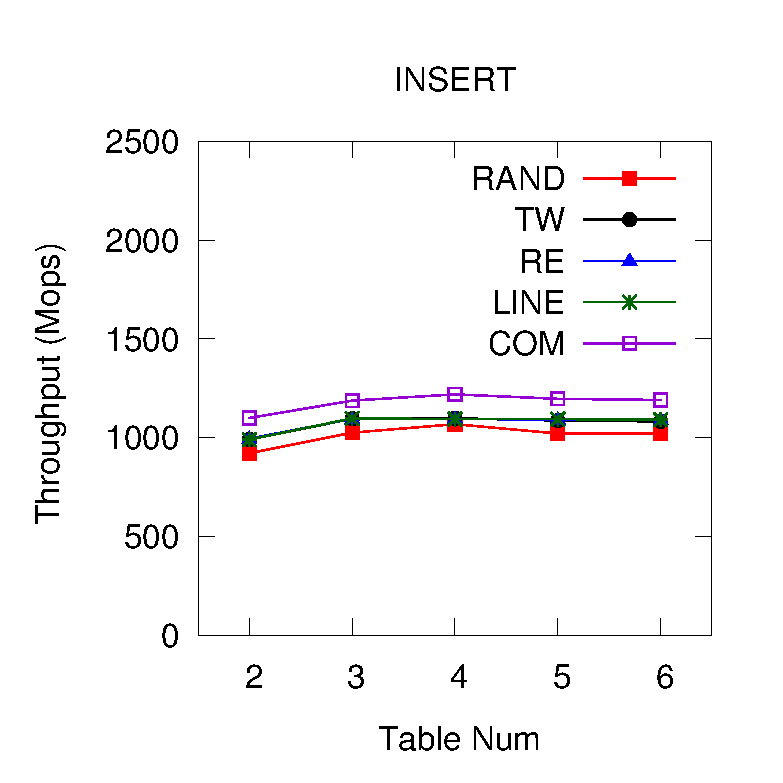
\includegraphics[width=\linewidth]{pic/tunning/tunning-insert.eps}
	\centerline{\formal{insert}}
	\end{minipage}
	\hfill
	\begin{minipage}{0.45\linewidth}\centering
	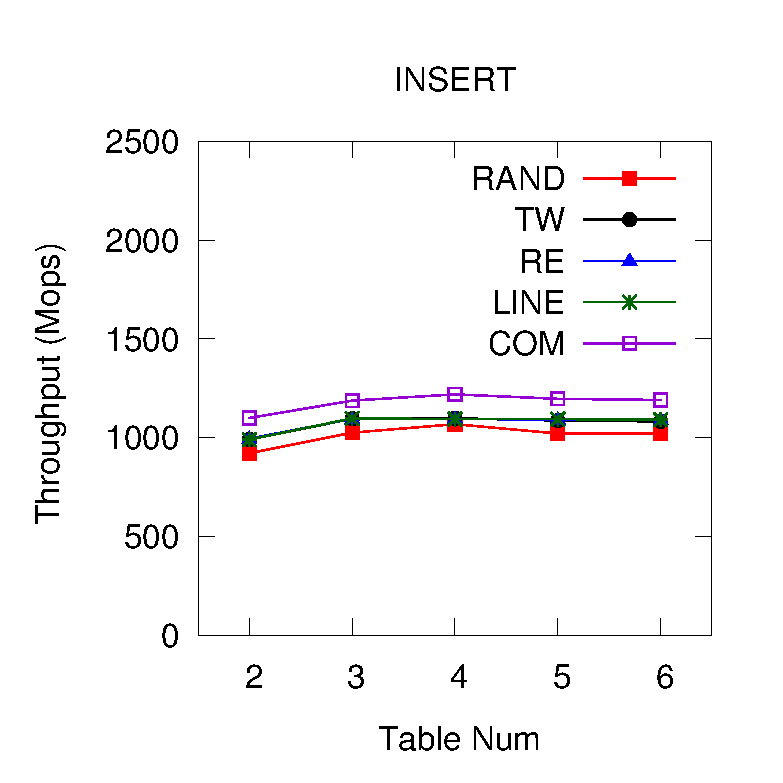
\includegraphics[width=\linewidth]{pic/tunning/tunning-insert.eps}
	\centerline{\formal{find}}
	\end{minipage}
	\caption{Throughput of \voter when varying number of hash tables.}
	\label{fig:vary-table}
\end{figure}

\subsection{Static Hashing Comparison}\label{sec:exp:static}
\vspace{1mm}\noindent\textbf{Varying the data variance $\sigma$.}

\begin{figure}[h]
	\begin{minipage}{0.45\linewidth}\centering
	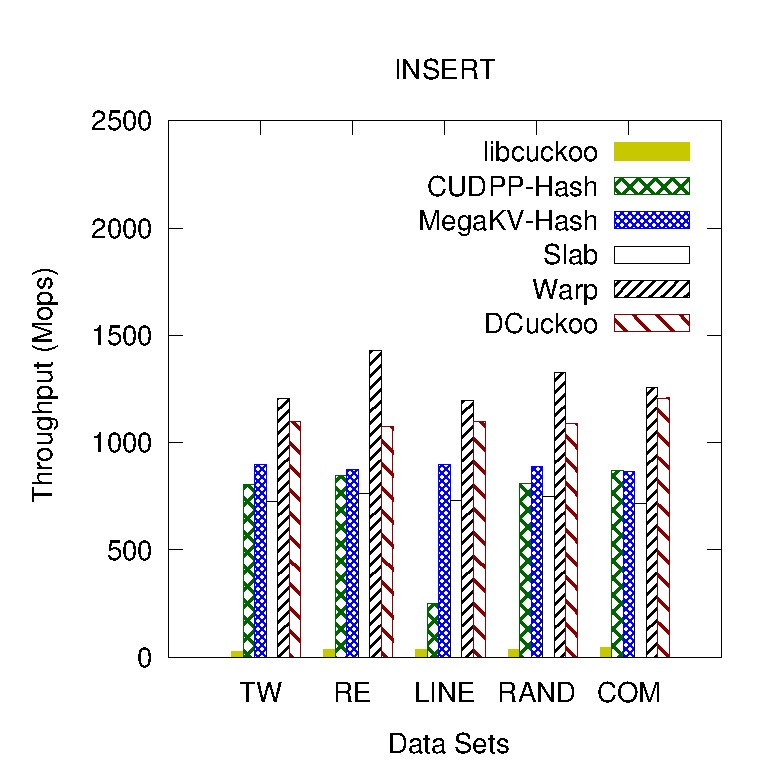
\includegraphics[width=\linewidth]{pic/static/static_insert.eps}
	\centerline{\formal{insert}}
	\end{minipage}
	\hfill
	\begin{minipage}{0.45\linewidth}\centering
	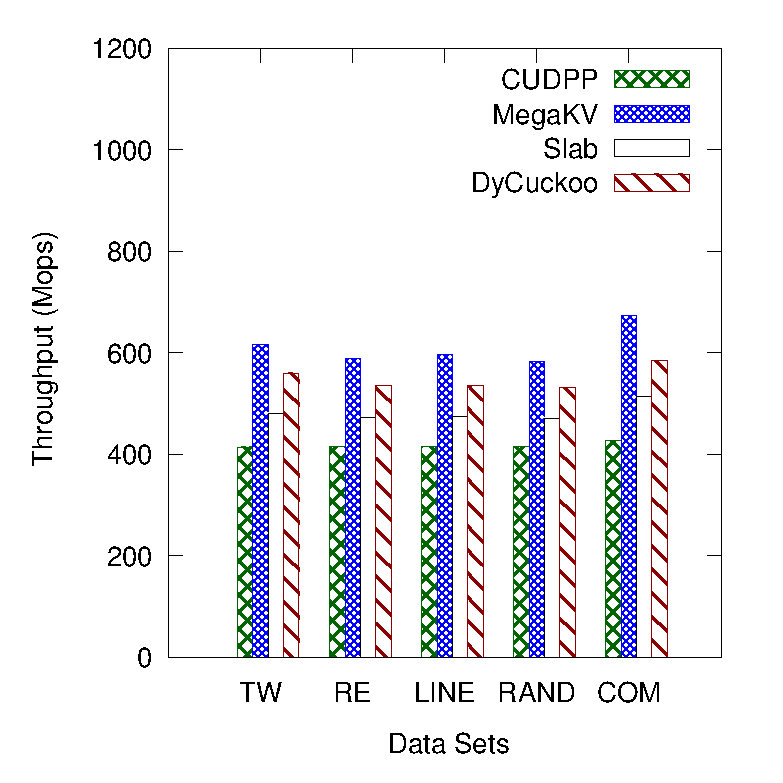
\includegraphics[width=\linewidth]{pic/static/static_search.eps}
	\centerline{\formal{find}}
	\end{minipage}
	\caption{Throughput of all compared approaches under the static setting.}
	\label{fig:static}
\end{figure}

\begin{figure*}[h]
	\begin{minipage}{0.3\linewidth}\centering
		\includegraphics[width=\linewidth]{fig/PlaceHolder.pdf}
		\centerline{Warp Efficiency}
	\end{minipage}
	\hfill
	\begin{minipage}{0.3\linewidth}\centering
	\includegraphics[width=\linewidth]{fig/PlaceHolder.pdf}
	\centerline{Memory Bandwidth Utilization}
	\end{minipage}
	\hfill
	\begin{minipage}{0.3\linewidth}\centering
	\includegraphics[width=\linewidth]{fig/PlaceHolder.pdf}
	\centerline{Cache Utilization}
	\end{minipage}
	\caption{Profiling the \formal{insert} performance for all compared approaches when varying the standard deviation $\sigma$.}
	\label{fig:static}
\end{figure*}

\subsection{Dynamic Hashing Comparison}\label{sec:exp:dynamic}

\vspace{1mm}\noindent\textbf{Varying the filled factor lower bound $\alpha$.}

\begin{figure*}[h]
	\begin{minipage}{0.18\linewidth}\centering
		\includegraphics[width=\linewidth]{fig/PlaceHolder.pdf}
		\centerline{\dstwitter}
	\end{minipage}
	\hfill
	\begin{minipage}{0.18\linewidth}\centering
		\includegraphics[width=\linewidth]{fig/PlaceHolder.pdf}
		\centerline{\dsreddit}
	\end{minipage}
	\hfill
	\begin{minipage}{0.18\linewidth}\centering
		\includegraphics[width=\linewidth]{fig/PlaceHolder.pdf}
		\centerline{\dstpch}
	\end{minipage}
	\hfill
	\begin{minipage}{0.18\linewidth}\centering
		\includegraphics[width=\linewidth]{fig/PlaceHolder.pdf}
		\centerline{\dsali}
	\end{minipage}
	\hfill
	\begin{minipage}{0.18\linewidth}\centering
		\includegraphics[width=\linewidth]{fig/PlaceHolder.pdf}
		\centerline{\dsrandom}
	\end{minipage}
	\caption{Run time for varying $\alpha$.}
	\label{fig:vary-alpha-time}
\end{figure*}

\begin{figure*}[h]
	\begin{minipage}{0.18\linewidth}\centering
		\includegraphics[width=\linewidth]{fig/PlaceHolder.pdf}
		\centerline{\dstwitter}
	\end{minipage}
	\hfill
	\begin{minipage}{0.18\linewidth}\centering
		\includegraphics[width=\linewidth]{fig/PlaceHolder.pdf}
		\centerline{\dsreddit}
	\end{minipage}
	\hfill
	\begin{minipage}{0.18\linewidth}\centering
		\includegraphics[width=\linewidth]{fig/PlaceHolder.pdf}
		\centerline{\dstpch}
	\end{minipage}
	\hfill
	\begin{minipage}{0.18\linewidth}\centering
		\includegraphics[width=\linewidth]{fig/PlaceHolder.pdf}
		\centerline{\dsali}
	\end{minipage}
	\hfill
	\begin{minipage}{0.18\linewidth}\centering
		\includegraphics[width=\linewidth]{fig/PlaceHolder.pdf}
		\centerline{\dsrandom}
	\end{minipage}
	\caption{System stability for varying $\alpha$.}
	\label{fig:vary-alpha-stability}
\end{figure*}

\vspace{1mm}\noindent\textbf{Varying the filled factor upper bound $\beta$.}

\begin{figure*}[h]
	\begin{minipage}{0.18\linewidth}\centering
		\includegraphics[width=\linewidth]{fig/PlaceHolder.pdf}
		\centerline{\dstwitter}
	\end{minipage}
	\hfill
	\begin{minipage}{0.18\linewidth}\centering
		\includegraphics[width=\linewidth]{fig/PlaceHolder.pdf}
		\centerline{\dsreddit}
	\end{minipage}
	\hfill
	\begin{minipage}{0.18\linewidth}\centering
		\includegraphics[width=\linewidth]{fig/PlaceHolder.pdf}
		\centerline{\dstpch}
	\end{minipage}
	\hfill
	\begin{minipage}{0.18\linewidth}\centering
		\includegraphics[width=\linewidth]{fig/PlaceHolder.pdf}
		\centerline{\dsali}
	\end{minipage}
	\hfill
	\begin{minipage}{0.18\linewidth}\centering
		\includegraphics[width=\linewidth]{fig/PlaceHolder.pdf}
		\centerline{\dsrandom}
	\end{minipage}
	\caption{Run time for varying $\beta$.}
	\label{fig:vary-beta-time}
\end{figure*}

\vspace{1mm}\noindent\textbf{Varying insert vs. delete ratio $r$.}

\begin{figure*}[h]
	\begin{minipage}{0.18\linewidth}\centering
		\includegraphics[width=\linewidth]{fig/PlaceHolder.pdf}
		\centerline{\dstwitter}
	\end{minipage}
	\hfill
	\begin{minipage}{0.18\linewidth}\centering
		\includegraphics[width=\linewidth]{fig/PlaceHolder.pdf}
		\centerline{\dsreddit}
	\end{minipage}
	\hfill
	\begin{minipage}{0.18\linewidth}\centering
		\includegraphics[width=\linewidth]{fig/PlaceHolder.pdf}
		\centerline{\dstpch}
	\end{minipage}
	\hfill
	\begin{minipage}{0.18\linewidth}\centering
		\includegraphics[width=\linewidth]{fig/PlaceHolder.pdf}
		\centerline{\dsali}
	\end{minipage}
	\hfill
	\begin{minipage}{0.18\linewidth}\centering
		\includegraphics[width=\linewidth]{fig/PlaceHolder.pdf}
		\centerline{\dsrandom}
	\end{minipage}
	\caption{Run time for varying $r$.}
	\label{fig:vary-r-time}
\end{figure*}

\vspace{1mm}\noindent\textbf{Varying the batch size.}

\begin{figure*}[h]
	\begin{minipage}{0.18\linewidth}\centering
		\includegraphics[width=\linewidth]{fig/PlaceHolder.pdf}
		\centerline{\dstwitter}
	\end{minipage}
	\hfill
	\begin{minipage}{0.18\linewidth}\centering
		\includegraphics[width=\linewidth]{fig/PlaceHolder.pdf}
		\centerline{\dsreddit}
	\end{minipage}
	\hfill
	\begin{minipage}{0.18\linewidth}\centering
		\includegraphics[width=\linewidth]{fig/PlaceHolder.pdf}
		\centerline{\dstpch}
	\end{minipage}
	\hfill
	\begin{minipage}{0.18\linewidth}\centering
		\includegraphics[width=\linewidth]{fig/PlaceHolder.pdf}
		\centerline{\dsali}
	\end{minipage}
	\hfill
	\begin{minipage}{0.18\linewidth}\centering
		\includegraphics[width=\linewidth]{fig/PlaceHolder.pdf}
		\centerline{\dsrandom}
	\end{minipage}
	\caption{Run time for varying the batch size.}
	\label{fig:vary-batch-size}
\end{figure*}

\section{conclusion}\label{sec:con}
In this paper, we contribute a number of novel designs for dynamic hash table on GPUs. 
First, we introduced an efficient strategy to resize only one of a subtable at a time. Our theoretical analysis demonstrated the near-optimality of the resizing strategy. Second, we devised a two-layer cuckoo has scheme that ensures at most two loops for find and deletion operations, while still retains similar performance for insertion as general cuckoo hash tables. 
Empirically, our proposed design achieves competitive performance against the state-of-the-art static GPU hash tables. Our hash table design achieves superior performance while saves up to 4x memory over the state-of-the-art approaches against dynamic workloads.

 



%

\section*{Appendix}

\begin{figure*}[t]
	\begin{minipage}{0.19\linewidth}\centering
		\includegraphics[width=\linewidth]{pic/static-upper/upper_insert_twitter.eps}
		\centerline{\dstwitter}
	\end{minipage}
	\hfill
	\begin{minipage}{0.19\linewidth}\centering
		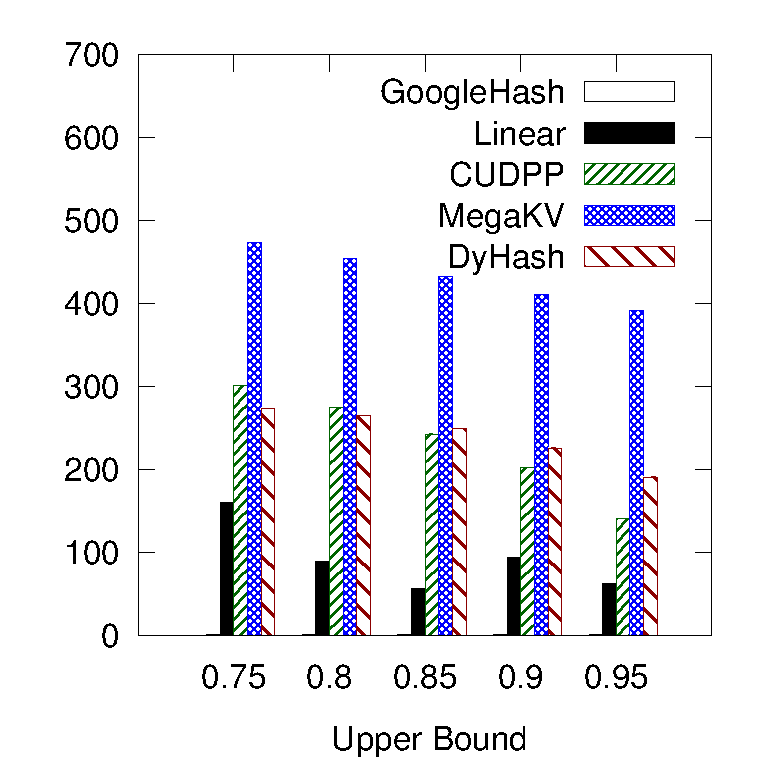
\includegraphics[width=\linewidth]{pic/static-upper/upper_insert_reddit.eps}
		\centerline{\dsreddit}
	\end{minipage}
	\hfill
	\begin{minipage}{0.19\linewidth}\centering
		\includegraphics[width=\linewidth]{pic/static-upper/upper_insert_tpch.eps}
		\centerline{\dstpch}
	\end{minipage}
	\hfill
	\begin{minipage}{0.19\linewidth}\centering
		\includegraphics[width=\linewidth]{pic/static-upper/upper_insert_ali.eps}
		\centerline{\dsali}
	\end{minipage}
	\hfill
	\begin{minipage}{0.19\linewidth}\centering
		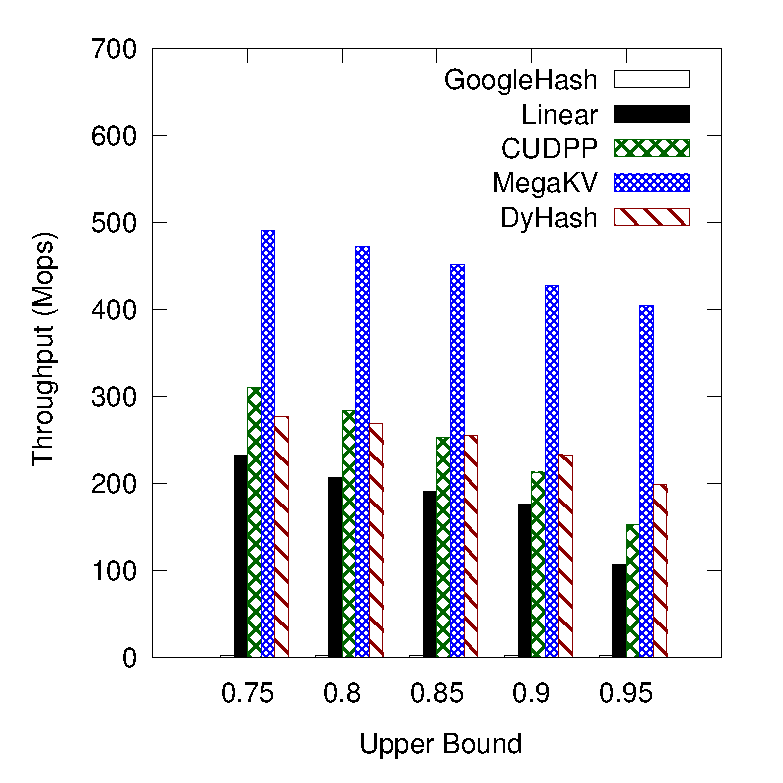
\includegraphics[width=\linewidth]{pic/static-upper/upper_insert_random.eps}
		\centerline{\dsrandom}
	\end{minipage}
	\caption{Throughputs of insert for varying $\beta$.}
	\label{fig:static:all:insert}
\end{figure*}
\begin{figure*}[t]
	\begin{minipage}{0.19\linewidth}\centering
		\includegraphics[width=\linewidth]{pic/static-upper/upper_search_twitter.eps}
		\centerline{\dstwitter}
	\end{minipage}
	\hfill
	\begin{minipage}{0.19\linewidth}\centering
		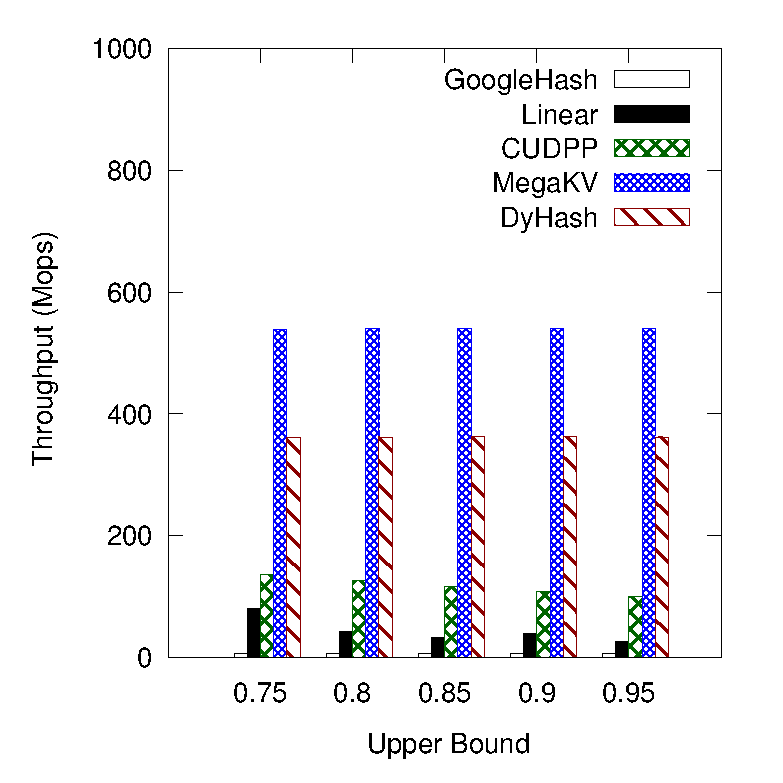
\includegraphics[width=\linewidth]{pic/static-upper/upper_search_reddit.eps}
		\centerline{\dsreddit}
	\end{minipage}
	\hfill
	\begin{minipage}{0.19\linewidth}\centering
		\includegraphics[width=\linewidth]{pic/static-upper/upper_search_tpch.eps}
		\centerline{\dstpch}
	\end{minipage}
	\hfill
	\begin{minipage}{0.19\linewidth}\centering
		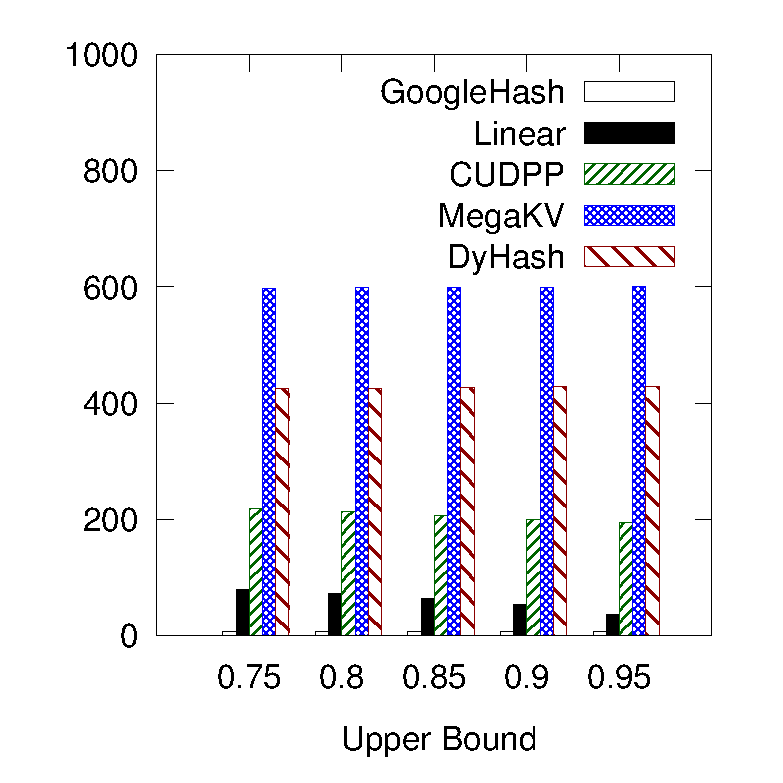
\includegraphics[width=\linewidth]{pic/static-upper/upper_search_ali.eps}
		\centerline{\dsali}
	\end{minipage}
	\hfill
	\begin{minipage}{0.19\linewidth}\centering
		\includegraphics[width=\linewidth]{pic/static-upper/upper_search_random.eps}
		\centerline{\dsrandom}
	\end{minipage}
	\caption{Throughputs of search for varying $\beta$.}
	\label{fig:static:all:search}
\end{figure*}




%\pagebreak
\bibliographystyle{abbrv}
\bibliography{ref}

\begin{IEEEbiography}[{\includegraphics[width=1in,height=1.25in,clip,keepaspectratio]{photos/yuchen.pdf}}]
	{Yuchen Li} is an assistant professor at the School of Information Systems, Singapore Management University (SMU).
	%Before joining SMU, he was a research fellow in the School of Computing, National University of Singapore (NUS).
	He received the double B.Sc. degrees in applied math and computer science (both degrees with first class honors)
	and the Ph.D. degree in computer science from NUS, in 2013 and 2016, respectively. He received the Lee Kong Chian Fellowship in 2019 for research excellence.
	His research interests include heterogeneous computing, graph analytics and computational journalism.
\end{IEEEbiography}

\begin{IEEEbiography}[{\includegraphics[width=1in,height=1.25in,clip,keepaspectratio]{photos/zhangjing.pdf}}]
	{Jing Zhang} is currently a graduate student at the College of Computer Science and Technology, Zhejiang University (ZJU). He received his B.Sc. from Huazhong University of Science and Technology (HUST) in 2017. His research interests include heterogeneous computing and data management.
\end{IEEEbiography}

\begin{IEEEbiography}[{\includegraphics[width=1in,height=1.25in,clip,keepaspectratio]{photos/liuyue.pdf}}]
	{Yue Liu} is currently a graduate student at the College of Computer Science and Technology, Zhejiang University (ZJU). She received her B.Eng. in the Internet of Things from Hunan University (HNU) in 2017. Her research interests include heterogeneous computing and data management.
\end{IEEEbiography}

\begin{IEEEbiography}[{\includegraphics[width=1in,height=1.25in,clip,keepaspectratio]{photos/lvzheng.pdf}}]
	{Zheng Lyu} is now a staff engineer at Alibaba group, and responsible for development of GPU databases. He received his PhD in communication and information system from Shanghai institute of microsystem and information technology, Chinese Academy of Sciences in 2012. He mainly works in the area of high performance computing and his major research interest is heterogeneous computing in database system.
\end{IEEEbiography}

\begin{IEEEbiography}[{\includegraphics[width=1in,height=1.25in,clip,keepaspectratio]{photos/huang.pdf}}]
	{Zhongdong Huang} is an associate professor in the College of Computer Science and Technology, Zhejiang University. He received his B.Sc in Telecommunication and PhD degree in Computer Science from Zhejiang University in 1989 and 2003 respectively. His research interests include big data analytics and database systems.
\end{IEEEbiography}

\begin{IEEEbiography}[{\includegraphics[width=1in,height=1.25in,clip,keepaspectratio]{photos/sun.pdf}}]
	{Jianling Sun} is a professor at the School of Computer Science and Technology. He received his PhD degree in computer science from Zhejiang University, China in 1993. His research interests include database systems, distributed computing, and machine Learning. He currently serves as the director of the Lab of Next Generation Database Technologies of Alibaba-Zhejiang University Joint Institute of Frontier Technologies. 
\end{IEEEbiography}


\end{document}
